\documentclass[UTF8,fontset=ubuntu]{ctexbook}
\usepackage{amsmath}
\usepackage{amssymb}
\usepackage{bm}
\usepackage{cancel}
\usepackage{colortbl}
\usepackage{float}
\usepackage{framed}
\usepackage[framed]{ntheorem}
\usepackage{parskip}
\usepackage{pifont}
\usepackage{tikz}
\usepackage{xcolor}
\usepackage[Bjornstrup]{fncychap}
\theoremheaderfont{\normalfont\bfseries}
\theorembodyfont{\slshape}
\theoremseparator{\hspace{2ex}}
\theoremindent2ex
\theoremstyle{plain}
\newtheorem{theorem}{定理}
\theoremstyle{nonumberplain}
\newtheorem{definition}{定义}
\theoremstyle{empty}
\newframedtheorem{law}{定律}
\definecolor{lightgray}{gray}{0.8}
\definecolor{gray}{gray}{0.6}
\definecolor{white}{gray}{1}
\renewcommand{\thesection}{}
\DeclareMathOperator{\Span}{Span}
\DeclareMathOperator{\Nul}{Nul}
\DeclareMathOperator{\Col}{Col}
\newcolumntype{R}{>{$}w{r}{4.5mm}<{$}}
\newcolumntype{B}{>{\columncolor{lightgray}[0pt]$}w{r}{4.5mm}<{$}}
\newcolumntype{W}{>{\columncolor{white}[0pt]$}w{r}{4.5mm}<{$}}
\begin{document}
\chapter{线性代数中的线性方程组}
\section{线性方程组}
包含变量$x_1,x_2,\cdots,x_n$的线性方程:
	\[ a_{1}x_{1}+a_{2}x_{2}+\cdots +a_{n}x_{n}=b \]
其中, $b$与系数$a_{1}$,$a_{2}$,$\cdots$,$a_{n}$是实数或复数, 通常为已知数. n为任意正整数\\[2ex]

线性方程组 -- 由一个或几个包含相同变量$x_1,x_2,\cdots,x_n$的线性方程组成, 如:
\[\begin{array}{r@{\hspace{1.5pt}}l@{\hspace{1.5pt}}r@{\hspace{1.5pt}}l@{\hspace{1.5pt}}r@{\hspace{1.5pt}}l@{\hspace{1.5pt}}r}
	2x_1 & - & x_2 & + & 1.5x_3 & = & 8\\
	x_1  &   &     & - & 4x_3   & = & -7		
\end{array}\]
若线性方程组的方程个数少于未知数个数, 称之为\textbf{欠定方程组}\\
若线性方程组的方程个数多余未知数个数, 称之为\textbf{超定方程组}\\[1ex]

方程组所有可能的解的集合称为线性方程组的\textbf{解集}\\
若两个方程组有相同的解集, 则这两个方程组称为\textbf{等价的}\\[2ex]

\begin{center}
\begin{boxedminipage}{8cm}
线性方程组的解有下列三种情况:\\
1.无解;\\
2.有唯一解;\\
3.有无穷多解.
\end{boxedminipage}
\end{center}\vspace{2ex}

当方程组有唯一解或无穷多解时, 称线性方程组\textbf{相容}; 当方程组无解时, 称线性方程组\textbf{不相容}\\[2ex]

线性方程组
\[\begin{array}{r@{\hspace{1.5pt}}l@{\hspace{1.5pt}}r@{\hspace{1.5pt}}l@{\hspace{1.5pt}}r@{\hspace{1.5pt}}l@{\hspace{1.5pt}}r}
x_1 & - & 2x_2 & + &  x_3 & = & 0\\
	& 	& 2x_2 & - & 8x_3 & = & 8\\
-4x_1 & + & 5x_2 & + & 9x_3 & = & -9
\end{array}\]

线性方程组的\textbf{系数矩阵}
\[\left[\begin{array}{r r r}
	1 & -2 & 1\\
	0 & 2  & -8\\
	-4 & 5 & 9
\end{array}\right]\]

线性方程组的\textbf{增广矩阵}
\[\left[\begin{array}{r r r r}
	1 & -2 & 1 & 0\\
	0 & 2  & -8 & 8\\
	-4 & 5 & 9 & -9
\end{array}\right]\]\\[2ex]

矩阵的\textbf{维数}说明它包含的行数和列数. 如: 当矩阵包含3行4列, 则维数为3$\times$4\\[2ex]

\begin{center}
\begin{boxedminipage}{10cm}
初等行变换:\\
1.倍加变换 - 将某方程替换为它与另一方程倍数的和;\\
2.对换变换 - 交换两个方程的位置;\\
3.倍乘变换 - 方程的所有系数乘以一个非0实数.
\end{boxedminipage}
\end{center}

当其中一个矩阵可以经过一系列初等行变换称为另一个矩阵, 则称两个矩阵为\textbf{行等价的}\\

例1.解下列方程组\\
\[\begin{array}{r@{\hspace{1.5pt}}l@{\hspace{1.5pt}}r@{\hspace{1.5pt}}l@{\hspace{1.5pt}}r@{\hspace{1.5pt}}l@{\hspace{1.5pt}}r}
	x_1 & - & 2x_2 & + & x_3 & = & 0\\
	& & 2x_2 & - & 8x_3 & = & 8\\
	-4x_1 & + & 5x_2 & + & 9x_3 & = & -9
\end{array}\]
推导过程:\\
增广矩阵:\\
\[\left[\begin{array}{r r r r}
	1 & -2 & 1 & 0\\
	0 & 2 & -8 & 8\\
	5 & 0 & -5 & 10
\end{array}\right]\]
1)\ding{174}-5\ding{172}, 得:\\
\[\left[\begin{array}{r r r r r} 
	1 & -2 & 1 & 0\\
	0 & 2 & -8 & 8\\
	0 & 10 & -10 & 10
\end{array}\right]\]
2)$\frac{1}{2}$\ding{173}, 得:\\
\[\left[\begin{array}{r r r r r} 
	1 & -2 & 1 & 0\\
	0 & 1 & -4 & 4\\
	0 & 10 & -10 & 10
\end{array}\right]\]
3)\ding{174}-10\ding{172}, 得:\\
\[\left[\begin{array}{r r r r r} 
	1 & -2 & 1 & 0\\
	0 & 1 & -4 & 4\\
	0 & 0 & 30 & -30
\end{array}\right]\]
4)$\frac{1}{30}$\ding{174}, 得:\\
\[\left[\begin{array}{r r r r r} 
	1 & -2 & 1 & 0\\
	0 & 1 & -4 & 4\\
	0 & 0 & 1 & -1
\end{array}\right]\]
5)\ding{173}+4\ding{174}, 得:\\
\[\left[\begin{array}{r r r r r} 
	1 & -2 & 1 & 0\\
	0 & 1 & 0 & 0\\
	0 & 0 & 1 & -1
\end{array}\right]\]
6)\ding{172}-\ding{174}, 得:\\
\[\left[\begin{array}{r r r r r} 
	1 & -2 & 0 & 1\\
	0 & 1 & 0 & 0\\
	0 & 0 & 1 & -1
\end{array}\right]\]
7)\ding{172}+2\ding{173}, 得:\\
\[\left[\begin{array}{r r r r r} 
	1 & 0 & 0 & 1\\
	0 & 1 & 0 & 0\\
	0 & 0 & 1 & -1
\end{array}\right]\]
方程组的解:(1,0,-1)\\[1ex]

例2.确定方程组是否相容\\
\[\begin{array}{r@{\hspace{1.5pt}}l@{\hspace{1.5pt}}r@{\hspace{1.5pt}}l@{\hspace{1.5pt}}r@{\hspace{1.5pt}}l@{\hspace{1.5pt}}r}
	& & x_2 & - & 4x_3 & = & 8\\
	2x_1& - & 3x_2 & + & 2x_3 & = & 1\\
	4x_1 & - & 8x_2 & + & 12x_3 & = & 1
\end{array}\]
推导过程:\\
增广矩阵:\\
\[\left[\begin{array}{r r r r}
	0 & 1 & -4 & 8\\
	2 & -3 & 2 & 1\\
	4 & -8 & 12 & 1
\end{array}\right]\]
1)\ding{172}$\rightleftharpoons$\ding{173}, 得:\\
\[\left[\begin{array}{r r r r}
	2 & -3 & 2 & 1\\
	0 & 1 & -4 & 8\\
	4 & -8 & 12 & 1
\end{array}\right]\]
2)\ding{174}-2\ding{172}, 得:\\
\[\left[\begin{array}{r r r r}
	2 & -3 & 2 & 1\\
	0 & 1 & -4 & 8\\
	0 & -2 & 8 & -1
\end{array}\right]\]
3)\ding{174}+2\ding{173}, 得:\\
\[\left[\begin{array}{r r r r}
	2 & -3 & 2 & 1\\
	0 & 1 & -4 & 8\\
	0 & 0 & 0 & 15
\end{array}\right]\]
方程组不相容\\[1ex]

\begin{center}
\framebox{若两个线性方程组的增广矩阵是行等价的, 则它们具有相同的解集}
\end{center}
\newpage

\section{行化简与阶梯形矩阵}
非零行(列): 矩阵中至少包含一个非零元素的行(列)\\
先导元素: 该行最左边的非零元素\\
\begin{definition}
一个矩阵称为阶梯形, 若它有以下三个性质:\\
1.所有非零行在零行之上;\\
2.某一行先导元素的列位于上一行先导元素的右边;\\
3.某一先导元素所在列下方元素都是零;\\
若还满足以下性质, 则称为简化阶梯形:\\
4.每一非零行的先导元素是1;\\
5.每一先导元素是该元素所在列的唯一非零元素.
\end{definition}\vspace{2ex}

\begin{TheoremTwo}[简化阶梯形矩阵的唯一性]
每个矩阵行等价于唯一的简化阶梯形矩阵.
\end{TheoremTwo}\vspace{2ex}

若矩阵A行等价于阶梯形矩阵U, 则称U为A的\textbf{阶梯形}; 若U是简化阶梯形, 则称U为A的\textbf{简化阶梯形}. \\
RREF(Reduced Row-Echelon Form): 简化阶梯形\\
REF(Row-Echelon Form): 阶梯形\\[2ex]

\begin{definition}
矩阵A中的{\heiti 主元位置}是A中对应于它的阶梯形中先导元素的位置.{\heiti 主元列}是A中含有主元位置的列.
\end{definition}\vspace{2ex}

例1.将下列矩阵利用行变换转化为阶梯型
\[A=\left[
\begin{array}{r r r r r}
	0 & -3 & -6 & 4 & 9\\
	-1 & -2 & -1 & 3 & 1\\
	-2 & -3 & 0 & 3 & -1\\
	1 & 4 & 5 & -9 & -7
\end{array}
\right]\]
推导过程:\\
1)\ding{172}$\rightleftharpoons$\ding{175}, 得:\\
\[\left[
\begin{array}{r r r r r}
	1 & 4 & 5 & -9 & -7\\
	-1 & -2 & -1 & 3 & 1\\
	-2 & -3 & 0 & 3 & -1\\
	0 & -3 & -6 & 4 & 9
\end{array}
\right]\]
2)\ding{173}+\ding{172}, 得:\\
\[\left[
\begin{array}{r r r r r}
	1 & 4 & 5 & -9 & -7\\
	0 & 2 & 4 & -6 & -6\\
	-2 & -3 & 0 & 3 & -1\\
	0 & -3 & -6 & 4 & 9
\end{array}
\right]\]
3)\ding{174}+2\ding{172}, 得:\\
\[\left[
\begin{array}{r r r r r}
	1 & 4 & 5 & -9 & -7\\
	0 & 2 & 4 & -6 & -6\\
	0 & 5 & 10 & -15 & -15\\
	0 & -3 & -6 & 4 & 9
\end{array}
\right]\]
4)\ding{174}-$\frac{5}{2}$\ding{173}, 得:\\
\[\left[
\begin{array}{r r r r r}
	1 & 4 & 5 & -9 & -7\\
	0 & 2 & 4 & -6 & -6\\
	0 & 0 & 0 & 0 & 0\\
	0 & -3 & -6 & 4 & 9
\end{array}
\right]\]
5)\ding{174}$\rightleftharpoons$\ding{175}, 得:\\
\[\left[
\begin{array}{r r r r r}
	1 & 4 & 5 & -9 & -7\\
	0 & 2 & 4 & -6 & -6\\
	0 & -3 & -6 & 4 & 9\\
	0 & 0 & 0 & 0 & 0
\end{array}
\right]\]


基本变量: 位于主元列的变量\\
自由变量: 位于非主元列的变量\\[2ex]

\begin{TheoremTwo}[存在与唯一性定理]
线性方程组相容的充要条件是增广矩阵的最右列不是主元列. 也就是说, 增广矩阵的阶梯形没有形如
	\[[0\ \cdots\ 0\ b], b\neq 0\]
的行. 若线性方程组相容, 则它的解集可能有两种情形:\\
1)当没有自由变量时, 有唯一解;\\
2)若至少有一个自由变量, 则有无穷多解.
\end{TheoremTwo}\vspace{2ex}

应用行化简算法解线性方程组:\\
1.写出方程组的增广矩阵\\
2.应用行化简算法把增广矩阵化为阶梯形, 确定方程组是否相容, 如果没有解则停止; 否则进行下一步\\
3.继续行化简算法得到它的简化阶梯形\\
4.写出简化阶梯形矩阵对应的方程组\\
5.将每个非零方程改写为使用自由变量表示基本变量的形式
\newpage

\section{向量方程}
仅含一列的矩阵称为列向量, 简称为向量. 包含两个元素得向量如下:
\[u=\left[\begin{array}{r}
	3\\
	-1
\end{array}\right] \text{\quad or\quad} u=(3, -1)\]\\[1ex]
所有两个元素的向量表示为$\mathbb{R}^2$, $\mathbb{R}$表示向量中的元素为实数, 2表示向量包含两个元素\\[1ex]

向量相等:\\
两个向量相等当且仅当其对应元素相等\\[1ex]

向量加法:\\
将向量的对应元素相加
\begin{equation*}
\left[\begin{array}{c}
	1\\
	-2
\end{array}\right]
+
\left[\begin{array}{c}
	2\\
	5
\end{array}\right]
=
\left[\begin{array}{c}
	1+2\\
	-2+5
\end{array}\right]
=
\left[\begin{array}{c}
	3\\
	3
\end{array}\right]
\end{equation*}

标量乘法:\\
将向量的元素乘以系数\\
\indent 若$u=\left[\begin{array}{c}3\\-1\end{array}\right]$, $c=5$, 则:
\[cu=5\left[\begin{array}{c}3\\-1\end{array}\right]=\left[\begin{array}{c}15\\-5\end{array}\right]\]

向量$\left[\begin{array}{r}x\\y\end{array}\right]$的几何含义: 由原点(0,0)指向点(x,y)的有向线段\\[2ex]

\begin{law}[向量加法的平行四边形法则]\ \\
若$\mathbb{R}^2$中向量$\mathbf{u}$和$\mathbf{v}$用平面上的点表示, 则$\mathbf{u+v}$对应于以$\mathbf{u}$,$\mathbf{0}$和$\mathbf{v}$为三个顶点的平行四边形的第4个顶点, 如图.\\[2ex]
\begin{center}
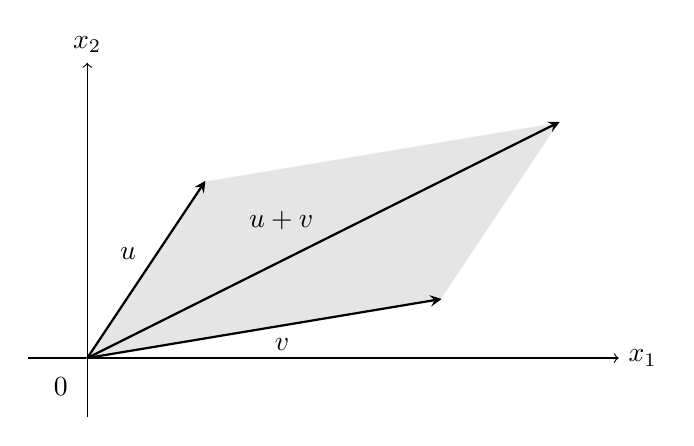
\begin{tikzpicture}[scale=0.75]
\draw[->] (-1,0) -- (9,0) node[right]{$x_1$};
\draw[->] (0,-1) -- (0,5) node[above]{$x_2$};
\draw[color=white, fill=black!10] (0,0) -- (6,1) -- (8,4) -- (2,3) -- cycle;
\draw[-stealth, thick, auto] (0,0) -- (2,3) node[pos=0.5]{$u$};
\draw[-stealth, thick, auto, swap] (0,0) -- (6,1) node[pos=0.5]{$v$};
\draw[-stealth, thick, auto] (0,0) -- (8,4) node[pos=0.5]{$u+v$};
\node at (0,0) [label=below left:$0$]{};
\end{tikzpicture}
\end{center}
\end{law}\vspace{3ex}

所有元素都是零的向量称为\textbf{零向量}, 用\textbf{0}表示(\textbf{0}中元素的个数可由上下文确定)\\[2ex]

\begin{law}[$\mathbb{R}^n$中向量的代数性质]\ \\
对$\mathbb{R}^n$中一切向量$\mathbf{u}$,$\mathbf{v}$,$\mathbf{w}$以及标量$c$和$d$:
\begin{equation*}
\begin{array}{l@{}c@{}l l l@{}c@{}l l}
( & i & ) & \mathbf{u}+\mathbf{v}=\mathbf{v}+\mathbf{u} & ( & v & ) & c(\mathbf{u}+\mathbf{v})=c\mathbf{u}+c\mathbf{v}\\
( & ii & ) & (\mathbf{u}+\mathbf{v})+\mathbf{w}=\mathbf{u}+(\mathbf{v}+\mathbf{w}) & ( & vi & ) & (c+d)\mathbf{u}=c\mathbf{u}+d\mathbf{u}\\
( & iii & ) & \mathbf{u}+\mathbf{0}=\mathbf{0}+\mathbf{u}=\mathbf{u} & ( & vii & ) & c(d\mathbf{u})=(cd)\mathbf{u}\\
( & iv & ) & \mathbf{u}+(-\mathbf{u})=-\mathbf{u}+\mathbf{u}=\mathbf{0} & ( & viii & ) & 1\mathbf{u}=\mathbf{u}
\end{array}
\end{equation*}
\end{law}\vspace{2ex}

给定$\mathbb{R}^n$中向量$\mathbf{v}_1$,$\mathbf{v}_2$,$\cdots$,$\mathbf{v}_p$和标量$c_1$,$c_2$,$\cdots$,$c_p$, 向量
	\[\mathbf{y}=c_1\mathbf{v}_1+\cdots+c_p\mathbf{v}_p\]
称为向量$\mathbf{v}_1$,$\mathbf{v}_2$,$\cdots$,$\mathbf{v}_p$以$c_1$,$c_2$,$\cdots$,$c_p$为\textbf{权}的\textbf{线性组合}.\\[2ex]

\framebox{
\begin{minipage}{\linewidth}
向量方程
\[x_1\mathbf{a}_1+x_2\mathbf{a}_2+\cdots+x_n\mathbf{a}_n=\mathbf{b}\]
和增广矩阵为
\begin{equation}
[\mathbf{a}_1\quad\mathbf{a}_2\quad\cdots\quad\mathbf{a}_n\quad\mathbf{b}]\label{matrix:eq_01}
\end{equation}
的线性方程组有相同的解集. 特别地, $\mathbf{b}$可表示为$\mathbf{a}_1$,$\mathbf{a}_2$,$\cdots$,$\mathbf{a}_n$的线性组合当且仅当对应于\eqref{matrix:eq_01}式的线性方程组有解.
\end{minipage}}\\[4ex]

\begin{definition}
若$\mathbf{v}_1$,$\mathbf{v}_2$,$\cdots$,$\mathbf{v}_p$是$\mathbb{R}^n$中的向量, 则$\mathbf{v}_1$,$\mathbf{v}_2$,$\cdots$,$\mathbf{v}_p$的所有线性组合所成的组合用记号$\Span\{\mathbf{v}_1$,$\mathbf{v}_2$,$\cdots$,$\mathbf{v}_p\}$表示, 称为由$\mathbf{v}_1$,$\mathbf{v}_2$,$\cdots$,$\mathbf{v}_p$所\textbf{生成}(或\textbf{张成})\textbf{的$\mathbb{R}^n$的子集}. 也就是说, $\Span\{\mathbf{v}_1$,$\mathbf{v}_2$,$\cdots$,$\mathbf{v}_p\}$是所有形如
	\[c_1\mathbf{v}_1+c_2\mathbf{v}_2+\cdots+c_p\mathbf{v}_p\]
的向量的集合, 其中$c_1$,$c_2$,$\cdots$,$c_p$为标量.\\[2ex]
\end{definition}\vspace{4ex}

\section{矩阵方程$A\mathbf{x}=\mathbf{b}$}
\begin{definition}
若$A$是$m\times n$矩阵, 它的各列为$\bm{a}_1$,$\cdots$,$\bm{a}_n$. 若$\bm{x}$是$\mathbb{R}^n$中的向量, 则\textbf{$A$与$\bm{x}$的积}(记为$A\bm{x}$)就是\textbf{$A$的各列以$\bm{x}$中对应元素为权的线性组合}, 即
	\[A\bm{x}=[\bm{a}_1\ \bm{a}_2\ \cdots\ \bm{a}_n]\left[\begin{array}{c}x_1\\x_2\\\vdots\\x_n\end{array}\right]=x_1\bm{a}_1+x_2\bm{a}_2+\cdots+x_n\bm{a}_n\]
注意$A\bm{x}$仅当$A$的列数等于$\bm{x}$中的元素个数时才有意义.\\[2ex]
\end{definition}

\begin{TheoremOne}
若$A$是$m\times n$矩阵, 它的各列为$\bm{a}_1$,$\cdots$,$\bm{a}_n$, 而$\bm{b}$属于$\mathbb{R}^n$, 则矩阵方程
\[A\bm{x}=\bm{b}\]
与向量方程
\[x_1\bm{a}_1+x_2\bm{a}_2+\cdots+x_n\bm{a}_n=\bm{b}\]
有相同的解集. 它又与增广矩阵为
\[[\bm{a}_1\ \bm{a}_2\ \cdots\ \bm{a}_n\ \bm{b}]\]
的线性方程组有相同的解集.\\[2ex]
\end{TheoremOne}\vspace{2ex}

\begin{TheoremOne}
设$A$是$m\times n$矩阵, 则下列命题是逻辑上等价的. 也就是说, 对某个$A$, 它们都成立或者都不成立.\\
\begin{tabular}{l@{\,}l}
a. & 对$\mathbb{R}^m$中每个$\bm{b}$, 方程$A\bm{x}=\bm{b}$有解.\\
b. & $\mathbb{R}^m$中的每个$\bm{b}$都是$A$的列的一个线性组合.\\
c. & $A$的各列生成$\mathbb{R}^m$.\\
d. & $A$在每一行都有一个主元位置.\\[2ex]
\end{tabular}
\end{TheoremOne}\vspace{2ex}

\begin{law}[计算$A\bm{x}$的行---向量规则]\ \\
若乘积$A\bm{x}$有定义, 则$A\bm{x}$中的第$i$个元素是$A$的第$i$行元素与$\bm{x}$的相应元素乘积之和.
\end{law}\vspace{2ex}

矩阵的主对角线上元素为1, 其他位置上元素为0, 这个矩阵称为\textbf{单位矩阵}, 并记为$I$.\\
如果矩阵为$n\times n$单位矩阵, 记为$I_n$.\\[2ex]

\begin{TheoremOne}
若$A$是$m\times n$矩阵, $\bm{u}$和$\bm{v}$是$\mathbb{R}^n$中向量, c是标量, 则\\
\begin{tabular}{l@{\,}l}
a. & $A(\bm{u}+\bm{v})=A\bm{u}+A\bm{v}$\\
b. & $A(c\bm{u})=c(A\bm{u})$
\end{tabular}
\end{TheoremOne}\vspace{6ex}

\section{线性方程组的解集}
若线性方程组可写成
\[A\bm{x}=\bm{0}\]
的形式, 则称为\textbf{齐次线性方程组}. 其中, $A$是$m\times n$矩阵, $\bm{0}$是$\mathbb{R}^m$中的零向量.\\
齐次线性方程组至少有一个解, 即$\bm{x}=\bm{0}$($\mathbb{R}^n$中的零向量), 这个解称为它的\textbf{平凡解}.\\
如果有一个非零向量$\bm{x}$, 满足$A\bm{x}=\bm{0}$, 这个解称为它的\textbf{非平凡解}.\\[2ex]

\begin{law}
齐次方程$A\bm{x}=\bm{0}$有非平凡解当且仅当方程至少有一个自由变量.
\end{law}\vspace{2ex}

$\bm{x}=s\bm{u}+t\bm{v}$为$A\bm{x}=\bm{0}$的\textbf{参数向量形式}, 并称之为\textbf{参数向量方程}. 其中, $s$,$t$为自由变量\\
$\bm{x}=\bm{p}+t\bm{v}$为$A\bm{x}=\bm{b}$的\textbf{参数向量形式}, 并称之为\textbf{参数向量方程}. 其中, $t$为自由变量\\
例.\\
$x_1=0.3x_2+0.2x_3$\\[1ex]
$\bm{x}=
\left[\begin{array}{l}
x_1\\
x_2\\
x_3
\end{array}\right]=
\left[\begin{array}{c}
0.3x_2+0.2x_3\\
x_2\\
x_3
\end{array}\right]=
\left[\begin{array}{r}
0.3x_2\\
x_2\\
0
\end{array}\right]+\left[\begin{array}{r}
0.2x_3\\
0\\
x_3
\end{array}\right]\\
\phantom{\bm{x}}=x_2\left[\begin{array}{r}
0.3\\
1\\
0
\end{array}\right]+x_3\left[\begin{array}{r}
0.2\\
0\\
1
\end{array}\right]
$\\[1ex]
因此, $A\bm{x}=\bm{b}$的解集是一条通过$\bm{p}$而平行于$A\bm{x}=\bm{0}$的解集的直线. 也称为将$\bm{v}$沿着$\bm{p}$进行直线移动.\\[2ex]

\begin{TheoremOne}
设方程$A\bm{x}=\bm{b}$对某个$\bm{b}$是相容的, $\bm{p}$为一个特解, 则$A\bm{x}=\bm{b}$的解集是所有形如$\bm{w}=\bm{p}+\bm{v}_h$的向量的集, 其中$\bm{v}_h$时齐次方程$A\bm{x}=\bm{b}$的任意一个解.
\end{TheoremOne}\vspace{3ex}

\begin{law}[把(相容方程组的)解集表示成参数向量形式]\ \\
1.把增广矩阵简化为简化阶梯形.\\
2.把每个基本变量用自由变量表示.\\
3.把一般解$\bm{x}$表示成向量, 如果有自由变量, 其元素依赖于自由变量.\\
4.把$\bm{x}$分解为向量(元素为常数)的线性组合, 用自由变量作为参数.
\end{law}\vspace{4ex}

\section{线性方程组的应用}
1.经济学 - 部分的收支平衡\\
2.化学式 - 等号两边原子守恒\\
3.网络流 - 节点的进/出流量恒等\\[4ex]

\section{线性无关}
\begin{definition}
$\mathbb{R}^n$中一组向量$\{\bm{v}_1$,$\cdots$,$\bm{v}_p\}$称为\textbf{线性无关}的, 若向量方程
\[x_1\bm{v}_1+x_2\bm{v}_2+\cdots+x_p\bm{v}_p=\bm{0}\]
仅有平凡解. 向量组(集)$\{\bm{v}_1$,$\cdots$,$\bm{v}_p\}$称为\textbf{线性相关}的, 若存在不全为零的权$c_1$,$\cdots$,$c_p$, 使
\[c_1\bm{v}_1+c_2\bm{v}_2+\cdots+c_p\bm{v}_p=\bm{0}\]
\end{definition}\vspace{2ex}

\begin{law}
矩阵$A$的各列线性无关, 当且仅当方程$A\bm{x}=\bm{0}$仅有平凡解.
\end{law}\vspace{2ex}

\begin{law}
两个向量的集合$\{\bm{v}_1$,$\bm{v}_2\}$线性相关, 当且仅当其中一个向量是另一个向量的倍数. 这个集合线性无关, 当且仅当其中任一个向量都不是另一个向量的倍数.
\end{law}\vspace{4ex}

\begin{TheoremTwo}[线性相关集的特征]
两个或更多个向量的集合$S=\{\bm{v}_1,\cdots,\bm{v}_p\}$线性相关, 当且仅当S中至少有一个向量是其他向量的线性组合. 事实上, 若S线性相关, 且$\bm{v}_1\neq\bm{0}$, 则某个$\bm{v}_j$$(j>1)$是它前面向量$\bm{v}_1$,$\cdots$,$\bm{v}_{j-1}$的线性组合.
\end{TheoremTwo}\vspace{4ex}

\begin{TheoremOne}
若一个向量组的向量个数超过每个向量的元素个数, 那么这个向量组线性相关. 就是说, $\mathbb{R}^n$中任意向量组$\{\bm{v}_1$,$\cdots$,$\bm{v}_p\}$当$p>n$时线性相关.
\end{TheoremOne}\vspace{4ex}

\begin{TheoremOne}
若$\mathbb{R}^n$中向量组$S=\{\bm{v}_1,\cdots,\bm{v}_p\}$包含零向量, 则它线性相关.
\end{TheoremOne}\vspace{4ex}

\section{线性变换介绍}
由$\bm{x}$到$A\bm{x}$的对应是由一个向量集到另一个向量集的函数\\[2ex]

\begin{definition}
变换(或映射)$T$称为\textbf{线性}的, 若\\
\begin{tabular}{l@{}c@{}l@{\hspace{2pt}}l}
$($ & i & $)$ & 对$T$的定义域中一切$\bm{u}$,$\bm{v}$,$T(\bm{u}+\bm{v})=T(\bm{u})+T(\bm{v})$.\\
$($ & ii & $)$ & 对$T$的定义域中的一切$\bm{u}$和数$c$, $T(c\bm{u})=cT(\bm{u})$.
\end{tabular}
\end{definition}\vspace{4ex}

\begin{law}
若T是线性变换, 则
\[T(\bm{0})=\bm{0}\]
且对$T$的定义域中一切向量$\bm{u}$和$\bm{v}$以及数$c$和$d$, 有:
\[T(c\bm{u}+d\bm{v})=cT(\bm{u})+dT(\bm{v})\]
\end{law}\vspace{6ex}

\section{线性变换的矩阵}
\begin{TheoremOne}
设$T$:$\mathbb{R}^n\rightarrow\mathbb{R}^m$为线性变换, 则存在唯一的矩阵$A$, 使得对$\mathbb{R}^n$中一切$\bm{x}$, 有
\[T(\bm{x})=A\bm{x}\]
事实上, $A$是$m\times n$矩阵, 它的第$j$列是向量$T(\bm{e}_j)$, 其中$\bm{e}_j$是$\mathbb{R}^n$中单位矩阵$\bm{I}_n$的第$j$列:
\[A=[T(\bm{e}_1)\ \cdots\ T(\bm{e}_n)]\]
\end{TheoremOne}\vspace{4ex}

\begin{definition}
映射$T$:$\mathbb{R}^n\rightarrow\mathbb{R}^m$称为到$\mathbb{R}^m$上的映射, 若$\mathbb{R}^m$中每个$\bm{b}$是$\mathbb{R}^n$中至少一个$\bm{x}$的像(也称为\textbf{满射}).
\end{definition}\vspace{4ex}

\begin{definition}
映射$T$:$\mathbb{R}^n\rightarrow\mathbb{R}^m$称为\textbf{一对一映射}(或1:1), 若$\mathbb{R}^m$中每个$\bm{b}$是$\mathbb{R}^n$中至多一个$\bm{x}$的像(也称为\text{单射}).
\end{definition}\vspace{4ex}

\begin{TheoremOne}
设$T$:$\mathbb{R}^n\rightarrow\mathbb{R}^m$为线性变换, 则$T$是一对一的当且仅当方程$A\bm{x}=\bm{0}$仅有平凡解.
\end{TheoremOne}\vspace{4ex}

\begin{TheoremOne}
设$T$:$\mathbb{R}^n\rightarrow\mathbb{R}^m$是线性变换, 设$A$为$T$的标准矩阵, 则\\
\begin{tabular}{l@{\ }l}
a. & $T$把$\mathbb{R}^n$映上到$\mathbb{R}^m$, 当且仅当$A$的列生成$\mathbb{R}^m$.\\
b. & $T$是一对一的, 当且仅当$A$的列线性无关.
\end{tabular}
\end{TheoremOne}\vspace{6ex}

\section{商业、科学和工程中的线性模型}
\begin{law}[基尔霍夫电压定律]\ \\
围绕一条回路同一方向的电压降$RI$的代数和等于围绕该回路的同一方向电动势的代数和.
\end{law}\vspace{4ex}

\begin{law}
如果有矩阵$A$使$\bm{x}_1=A\bm{x}_0$,$\bm{x}_2=A\bm{x}_1$, 一般地,
\[\bm{x}_{k+1}=A\bm{x}_k\text{,\ }k=0,1,2,\cdots\]
则称为\textbf{线性差分方程}(或\textbf{递归关系}).
\end{law}

% \documentclass[UTF8,fontset=ubuntu]{ctexart}
% \usepackage{amsmath}
% \usepackage{bm}
% \usepackage{parskip}
% \usepackage{amssymb}
% \usepackage{xcolor}
% \usepackage{colortbl}
% \usepackage{framed}
% \usepackage[framed]{ntheorem}
% \theoremheaderfont{\normalfont\bfseries}
% \theorembodyfont{\slshape}
% \theoremseparator{\hspace{2ex}}
% \theoremindent2ex
% \theoremstyle{plain}
% \newtheorem{theorem}{定理}
% \theoremstyle{nonumberplain}
% \newtheorem{definition}{定义}
% \theoremstyle{empty}
% \newframedtheorem{law}{定律}
% \definecolor{lightgray}{gray}{0.7}
% \definecolor{gray}{gray}{0.5}
% \definecolor{white}{gray}{1}
% \begin{document}
\part{矩阵代数}
\section{一、矩阵运算}
$m\times n$矩阵$A=[a_{ij}]$的\textbf{对角线元素}是$a_{11}$,$a_{22}$,$a_{33}$,$\cdots$, 它们组成$A$的\textbf{主对角线}.\\[1ex]
\textbf{对角矩阵}是一个方阵, 它的非对角线元素全是0. 例如$n\times n$单位矩阵$\bm{I}_n$.\\[1ex]
元素全是0的$m\times n$矩阵称为\textbf{零矩阵}, 用$\bm{0}$表示.\\[1ex]
若两个矩阵有相同的维数(即有相同的行数和列数), 而且对应元素相同, 则称该两个矩阵\textbf{相等}\\[1ex]
若$r$是标量而$A$是矩阵, 则\textbf{标量乘法}$rA$是一个矩阵, 它的每一列是$A$的对应列的$r$倍.\\[2ex]

\begin{theorem}
设$A$,$B$,$C$是相同维数的矩阵, $r$与$s$为数, 则有\\
\begin{tabular}{l@{\ }l@{\hspace{5em}}l@{\ }l}
a. & $A+B=B+A$ & b. & $(A+B)+C=A+(B+C)$\\
c. & $A+0=A$ & d. & $r(A+B)=rA+rB$\\
e. & $(r+s)A=rA+sA$ & f. & $r(sA)=(rs)A$
\end{tabular}
\end{theorem}\vspace{4ex}

\begin{definition}
若$A$是$m\times n$矩阵, $B$是$n\times p$矩阵, $B$的列是$\bm{b}_1$,$\cdots$,$\bm{b}_p$, 则乘积$AB$是$m\times p$矩阵, 它的各列是$A\bm{b}_1$,$\cdots$,$A\bm{b}_p$, 即
\[AB=A[\bm{b}_1\ \bm{b}_2\ \cdots\ \bm{b}_p]=[A\bm{b}_1\ A\bm{b}_2\ \cdots\ A\bm{b}_p]\]
\end{definition}\vspace{4ex}

\begin{law}
$AB$的每一列都是$A$的各列的线性组合, 以$B$的对应列的元素为权.
\end{law}\vspace{4ex}

\begin{law}[计算$AB$的行列法则]\ \\
若乘积$AB$有定义, 则$AB$的第$i$行第$j$列的元素是$A$的第$i$行与$B$的第$j$列对应元素乘积之和. 若($AB$)${}_{ij}$表示$AB$的($i$,$j$)元素, $A$为$m\times n$矩阵, 则
\[(AB)_{ij}=a_{i1}b_{1j}+a_{i2}b_{2j}+\cdots+a_{in}b_{nj}\]
\end{law}\vspace{4ex}

\begin{theorem}
设$A$为$m\times n$矩阵, $B$和$C$的维数使下列各式的乘积有意义.\\
\begin{tabular}{l@{\ }l l}
a. & $A(BC)=(AB)C$ & (乘法结合律)\\
b. & $A(B+C)=AB+AC$ & (乘法左分配律)\\
c. & $(B+C)A=BA+CA$ & (乘法右分配律)\\
d. & $r(AB)=(rA)B=A(rB)$, r为任意数 &\\
e. & $I_mA=A=AI_m$ & (矩阵乘法的恒等式)
\end{tabular}
\end{theorem}\vspace{4ex}

乘积$AB$的因子关系为: $A$被$B$\textbf{右乘}, 或$B$被$A$\textbf{左乘}\\
若$AB$=$BA$, 我们称$A$和$B$彼此\textbf{可交换}\\[2ex]

\textbf{警告}\\
1.一般情况下, $AB\neq BA$.\\
2.消去律对矩阵乘法不成立, 即若$AB=AC$, 一般情况下, $B=C$并不成立.\\
3.若乘积$AB$是零矩阵, 一般情况下, 不能断定A=0或B=0.\\[2ex]

给定$m\times n$矩阵, 则$A$的\textbf{转置}是一个$n\times m$矩阵, 用$A^T$表示, 它的列是由$A$的对应行构成的.\\[2ex]

\begin{theorem}
设$A$与$B$表示矩阵, 其维数使下列和与积有定义, 则\\
\begin{tabular}{l@{\ }l}
a. & $(A^T)^T=A$.\\
b. & $(A+B)^T=A^T+B^T$.\\
c. & 对任意数$r$, $(rA)^T=rA^T$.\\
d. & $(AB)^T=B^TA^T$.
\end{tabular}
\end{theorem}\vspace{4ex}

\begin{law}
若干个矩阵的乘积的转置等于它们的转置的乘积, 但相乘的顺序相反.
\end{law}\vspace{8ex}

\section{二、矩阵的逆}
$A$为$n\times n$矩阵, 若存在一个$n\times n$矩阵$C$, 使得
\[CA=\bm{I}_n\qquad\text{且}AC=\bm{I}_n\]
则称$A$\textbf{可逆}, 并且$C$是$A$的\textbf{逆}.\\[2ex]
若$A$可逆, 它的逆是唯一的, 我们将它记为$A^{-1}$, 则
\[A^{-1}A=I\qquad\text{且}AA^{-1}=I\]
不可逆矩阵也称为\textbf{奇异矩阵}.\\
可逆矩阵也称为\textbf{非奇异矩阵}.\\[2ex]

\begin{theorem}
设$A=\left[\begin{array}{r r}3 & 4\\5 & 6\end{array}\right]$. 若$ad-bc\neq 0$, 则$A$可逆且
\[A^{-1}=\frac{1}{ad-bc}\left[\begin{array}{l l}d & -b\\-c & a\end{array}\right]\]
若$ad-bc=0$, 则$A$不可逆.
\end{theorem}\vspace{4ex}

数$ad-bc$称为$A$的\textbf{行列式}, 记为
\[\det A=ad-bc\]\\

\begin{theorem}
若$A$是可逆$n\times n$矩阵, 则对每一$\mathbb{R}^n$中的$\bm{b}$, 方程$A\bm{x}=\bm{b}$有唯一解$\bm{x}=A^{-1}\bm{b}$.
\end{theorem}\vspace{4ex}

\begin{law}[胡克定律]\ \\
公式如下
\[\bm{y}=D\bm{f}\]
其中$D$为\textbf{弹性矩阵}, 它的逆称为\textbf{刚性矩阵}, $\bm{f}$表示它在各个点受的力, $\bm{y}$表示各个点的形变量.
\end{law}\vspace{4ex}

\begin{theorem}\ \\
a.若$A$是可逆矩阵, 则$A^{-1}$也可逆而且$(A^{-1})^{-1}=A$.\\
b.若$A$和$B$都是$n\times n$可逆矩阵, 则$AB$也可逆, 且其逆是$A$和$B$的逆矩阵按相反顺序的乘积, 即
\[(AB)^{-1}=B^{-1}A^{-1}\]
c.若$A$可逆, 则$A^T$也可逆, 且其逆是$A^{-1}$的转置, 即$(A^T)^{-1}=(A^{-1})^T$.
\end{theorem}\vspace{4ex}

\begin{law}
若干个$n\times n$可逆矩阵的积也是可逆的, 其逆等于这些矩阵的逆按相反顺序的乘积.
\end{law}\vspace{4ex}

把单位矩阵进行一次初等行变换, 就得到\textbf{初等矩阵}.\\[2ex]

\begin{law}
若对$m\times n$矩阵$A$进行某种初等行变换, 所得矩阵可写成$EA$, 其中$E$是$m\times m$矩阵, 是由$I_m$进行同一行变换所得.
\end{law}\vspace{4ex}

\begin{law}
每个初等矩阵$E$是可逆的, $E$的逆是一个同类型的初等矩阵, 它把$E$变回$I$.
\end{law}\vspace{4ex}

\begin{theorem}
$n\times n$矩阵$A$是可逆的, 当且仅当$A$行等价于$I_n$, 这时, 把$A$化简为$I_m$的一系列初等行变化同时把$I_n$变成$A^{-1}$.
\end{theorem}\vspace{4ex}

\begin{law}[求$A^{-1}$的算法]\ \\
把增广矩阵$[A\ I]$进行行化简. 若$A$行等价于$I$, 则$[A\ I]$行等价于$[I\ A^{-1}]$, 否则$A$没有逆.
\end{law}\vspace{8ex}

\section{三、可逆矩阵的特征}
\begin{theorem}[可逆矩阵定理]
设$A$为$n\times n$矩阵, 则下列命题是等价的, 即对某一特定的$A$, 它们同时为真或同时为假.\\
\begin{tabular}{l@{\ }l}
a. & $A$是可逆矩阵.\\
b. & $A$行等价于$n\times n$单位矩阵.\\
c. & $A$有$n$个主元位置.\\
d. & 方程$A\bm{x}=\bm{0}$仅有平凡解.\\
e. & $A$的各列线性无关.\\
f. & 线性变换$\bm{x}\mapsto A\bm{x}$是一对一的.\\
g. & 对$\mathbb{R}^n$中任意$\bm{b}$, 方程$A\bm{x}=\bm{b}$至少有一个解.\\
h. & $A$的各列生成$\mathbb{R}^n$,\\
i. & 线性变换$\bm{x}\mapsto A\bm{x}$把$\mathbb{R}^n$映上到$\mathbb{R}^n$.\\
j. & 存在$n\times n$矩阵$C$使$CA=I$.\\
k. & 存在$n\times n$矩阵$D$使$AD=I$.\\
l. & $A^T$是可逆矩阵.
\end{tabular}
\end{theorem}\vspace{4ex}

\begin{law}
设$A$和$B$为方阵, 若$AB=I$, 则$A$和$B$都是可逆的, 且$B=A^{-1}$, $A=B^{-1}$.
\end{law}\vspace{4ex}

\begin{theorem}
设$T$:$\mathbb{R}^n\rightarrow\mathbb{R}^n$为线性变换, $A$为$T$的标准矩阵. 则$T$可逆当且仅当$A$是可逆矩阵.
\end{theorem}\vspace{4ex}

若一个$m\times n$矩阵的主对角线以下元素全为0, 则称之为\textbf{上三角矩阵}.\\[1ex]
若一个$m\times n$矩阵的主对角线以上元素全为0, 则称之为\textbf{下三角矩阵}.\\[4ex]

\section{四、分块矩阵}
形如
\[A=\left[
\begin{array}{r r r|r r|r}
3 & 0 & -1 & 5 & 9 & -2\\
-5 & 2 & 4 & 0 & -3 & 1\\\hline
-8 & -6 & 3 & 1 & 7 & -4
\end{array}
\right]\]
为矩阵$A$的$2\times 3$\textbf{分块矩阵}, 也可表示为
\[A=\left[
\begin{array}{l l l}
A_{11} & A_{12} & A_{13}\\
A_{21} & A_{22} & A_{23}
\end{array}
\right]\]\\[2ex]

设$A$为$m\times n$矩阵, $B$为$n\times p$矩阵, 当$A$的列的分法与$B$的行的分法一致时, 可计算$AB$. 如下:
\[A=\left[\begin{array}{r r r|r r}
2 & -3 & 1 & 0 & -4\\
1 & 5 & -2 & 3 & -1\\\hline
0 & -4 & -2 & 7 & -1
\end{array}\right]=
\left[\begin{array}{l l}
A_{11} & A_{12}\\
A_{21} & A_{22}
\end{array}\right]\]
\[B=\left[\begin{array}{r r}
6 & 4\\
-2 & 1\\
-3 & 7\\\hline
-1 & 3\\
5 & 2
\end{array}\right]=
\left[\begin{array}{l}
B_1\\
B_2
\end{array}\right]\]
\[AB=\left[
\begin{array}{l l}
A_{11} & A_{12}\\
A_{21} & A_{22}
\end{array}
\right]\left[
\begin{array}{l}
B_1\\
B_2
\end{array}
\right]=\left[
\begin{array}{l}
A_{11}B_1+A_{12}B_2\\
A_{21}B_1+A_{22}B_2
\end{array}
\right]=\left[
\begin{array}{r r}
-5 & 4\\
-6 & 2\\\hline
2 & 1
\end{array}
\right]\]\\[2ex]

\begin{theorem}[$AB$的列行展开]\ \\
若$A$是$m\times n$矩阵, $B$是$n\times p$矩阵, 则
\[\begin{array}{l@{}l}
AB & =[col_1(A)\ col_2(A)\ \cdots\ col_n(A)]\left[
\begin{array}{c}
row_1(B)\\
row_2(B)\\
\vdots\\
row_n(B)
\end{array}
\right]\\
& =col_1(A)row_1(B)+\cdots+col_n(A)row_n(B)
\end{array}\]
\end{theorem}\vspace{8ex}

\section{五、矩阵因式分解}
设$A$是$m\times n$矩阵, 它可以行化简为阶梯形(化简步骤不包含对换变换), 则$A$可写成$A=LU$. 其中, $L$是$m\times m$下三角矩阵, 主对角线元素全是1; $U$是$A$的一个$m\times n$阶梯形矩阵.\\[2ex]

\begin{law}[$LU$分解的算法]\ \\
1.如果可能的话, 用一系列的行倍加变换把$A$化为阶梯形$U$(即$L^{-1}A=U$).\\
2.填充$L$的元素使相同的行变换把$L$变为$I$.
\end{law}\vspace{4ex}

$LU$分解图解:\\
\[\begin{array}{c@{}c@{}c@{}c@{}c@{}c@{}c@{}c@{}c}
A= & \left[\hspace{-1ex}\begin{array}{>{\columncolor{lightgray}[0pt]}r r r r}
\cellcolor{gray}2 & 4 & 5 & -2\\
-4 & -5 & -8 & 1\\
2 & -5 & 1 & 8\\
-6 & 0 & -3 & 1
\end{array}\hspace{-1ex}\right] & \Rightarrow & \left[\!\begin{array}{r >{\columncolor{white}[0pt]}r r r}
2 & 4 & 5 & -2\\
0 & \cellcolor{gray}3 & 2 & -3\\
0 & \cellcolor{lightgray}-9 & -4 & 10\\
0 & \cellcolor{lightgray}12 & 12 & -5
\end{array}\hspace{-1ex}\right] & \Rightarrow & \left[\!\begin{array}{r r >{\columncolor{white}[6pt][0pt]}r r}
2 & 4 & 5 & -2\\
0 & 3 & 2 & -3\\
0 & 0 & \cellcolor{gray}2 & 1\\
0 & 0 & \cellcolor{lightgray}4 & 7
\end{array}\hspace{-1ex}\right] & \Rightarrow & \left[\!\begin{array}{r r r >{\columncolor{white}[0pt]}r}
2 & 4 & 5 & -2\\
0 & 3 & 2 & -3\\
0 & 0 & 2 & 1\\
0 & 0 & 0 & \cellcolor{gray}5
\end{array}\hspace{-1ex}\right] & =U\\
& \downarrow & & \downarrow & & \downarrow & & \downarrow &\\
 & \left[\hspace{-1ex}\begin{array}{>{\columncolor{lightgray}[0pt]}r r r r}
\cellcolor{gray}1 & 0 & 0 & 0\\
-2 & 1 & 0 & 0\\
1 & & 1 & 0\\
-3 & & & 1
\end{array}\hspace{-1ex}\right] & & \left[\!\begin{array}{r >{\columncolor{white}[0pt]}r r r}
1 & 0 & 0 & 0\\
-2 & \cellcolor{gray}1 & 0 & 0\\
1 & \cellcolor{lightgray}-3 & 1 & 0\\
-3 & \cellcolor{lightgray}4 & & 1
\end{array}\hspace{-1ex}\right] & & \left[\!\begin{array}{r r >{\columncolor{white}[6pt][0pt]}r r}
1 & 0 & 0 & 0\\
-2 & 1 & 0 & 0\\
1 & -3 & \cellcolor{gray}1 & 0\\
-3 & 4 & \cellcolor{lightgray}2 & 1
\end{array}\hspace{-1ex}\right] & & \left[\!\begin{array}{r r r >{\columncolor{white}[6pt][0pt]}r}
1 & 0 & 0 & 0\\
-2 & 1 & 0 & 0\\
1 & -3 & 1 & 0\\
-3 & 4 & 2 & \cellcolor{gray}1
\end{array}\!\right] & =L
\end{array}\]\\[4ex]

\section{六、列昂惕夫投入产出模型}
\begin{law}[列昂惕夫投入产出模型或生产方程]\ \\
\[\bm{x}=C\bm{x}+\bm{d}\]
\end{law}\vspace{4ex}

\begin{theorem}
设$C$为某一经济体系的消耗矩阵, $\bm{d}$为最终需求. 若$C$和$\bm{d}$的元素非负, $C$的每一列的和小于1, 则$(I-C)^{-1}$存在, 产出向量
\[\bm{x}=(I-C)^{-1}\bm{d}\]
有非负元素, 且是下列方程的唯一解:
\[\bm{x}=C\bm{x}+d\]
\end{theorem}\vspace{8ex}

\section{七、计算机图形学中的应用}
物体的平移并不直接对应于矩阵乘法, 因为平移并非线性变换, 所以引入\textbf{齐次坐标}\\[1ex]
$\mathbb{R}^2$中每个点$(x,y)$对应于$\mathbb{R}^3$中的点$(x,y,1)$, $(x,y,1)$为$(x,y)$的\textbf{齐次坐标}\\[1ex]
$(x,y,1)\mapsto(x+h,y+k,1)$的平移变换实现:\\
\[\left[\begin{array}{r r r}
1 & 0 & h\\
0 & 1 & k\\
0 & 0 & 1
\end{array}\right]
\left[\begin{array}{r}
x\\
y\\
1
\end{array}\right]=
\left[\begin{array}{c}
x+h\\
y+k\\
1
\end{array}\right]\]\\[2ex]
$\mathbb{R}^2$中任意线性变换可以通过齐次坐标乘以分块矩阵$\left[\begin{array}{r r}A & 0\\0 & 1\end{array}\right]$实现, 其中$A$是$2\times 2$矩阵.\\[2ex]
$(x,y,z,1)$是$\mathbb{R}^3$中点$(x,y,z)$的齐次坐标. 若$H\neq 0$, 则$(X,Y,Z,H)$为$(x,y,z)$的齐次坐标, 且
\[x=\frac{X}{H},y=\frac{Y}{H},z=\frac{Z}{H}\]\\[1ex]
点$(x,y,z)$在$xy$平面上的透视投影坐标为$(\dfrac{x}{1-z/d}, \dfrac{y}{1-z/d}, 0)$. 其中, $d$为$z$轴观测位置$(0,0,d)$\\[2ex]
绕$\mathbb{R}^2$中一点$p$的旋转是这样实现的: 首先把图形平移$-p$, 然后绕原点旋转, 最后平移$p$.
% \end{document}

\documentclass[UTF8, fontset=ubuntu]{ctexart}
\usepackage{amsmath}
\usepackage{parskip}
\usepackage{cancel}
\begin{document}
一、行列式介绍\\[1ex]
有$3\times 3$矩阵$A$
\[\left[\begin{array}{l l l}
a_{11} & a_{12} & a_{13}\\
a_{21} & a_{22} & a_{23}\\
a_{31} & a_{32} & a_{33}
\end{array}\right]\]
其中
\[\Delta=a_{11}a_{22}a_{33}+a_{12}a_{23}a_{31}+a_{13}a_{21}a_{32}-a_{11}a_{23}a_{32}-a_{12}a_{21}a_{33}-a_{13}a_{22}a_{31}\]
$\Delta$称为$3\times 3$矩阵$A$的\textbf{行列式}, 也可以写成\\
$\Delta=(a_{11}a_{22}a_{33}-a_{11}a_{23}a_{32})-(a_{12}a_{21}a_{33}-a_{12}a_{23}a_{31})+(a_{13}a_{21}a_{32}-a_{13}a_{22}a_{31})$\\[1ex]
$\phantom{\Delta}=a_{11}\cdot\det\left[\begin{array}{l l}
a_{22} & a_{23}\\
a_{32} & a_{33}
\end{array}\right]-a_{12}\cdot\det\left[\begin{array}{l l}
a_{21} & a_{23}\\
a_{31} & a_{33}
\end{array}\right]+a_{13}\cdot\det\left[\begin{array}{l l}
a_{21} & a_{22}\\
a_{31} & a_{32}
\end{array}\right]$\\[1ex]
$\phantom{\Delta}=a_{11}\cdot\det A_{11}-a_{12}\cdot\det A_{12}+a_{13}\cdot\det A_{13}$\\
其中, $A_{ij}$表示去除矩阵第$i$行和第$j$列元素后的内容.\\
例. $A_{11}$表示如下:\\
\[\left[\begin{array}{l l l}
\cancel{a_{11}} & \cancel{a_{12}} & \cancel{a_{13}}\\
\cancel{a_{21}} & a_{22} & a_{23}\\
\cancel{a_{31}} & a_{32} & a_{33}
\end{array}\right]\]
即
\[\left[\begin{array}{l l}
a_{22} & a_{23}\\
a_{32} & a_{33}
\end{array}\right]\]
\end{document}

\chapter{向量空间}
\section{向量空间和子空间}
\begin{definition}
一个向量空间是由一些被称为向量的对象构成的非空集合V, 在这个集合上定义两个运算, 称为加法和标量乘法(标量取实数), 服从以下公理(或法则), 这些公理必须对V中所有向量$\mathbf{u}$,$\mathbf{v}$,$\mathbf{w}$及所有标量c和d均成立.\\
1.\quad$\mathbf{u}$,$\mathbf{v}$之和表示为$\mathbf{u}+\mathbf{v}$, 仍在V中\\
2.\quad$\mathbf{u+v=v+u}$\\
3.\quad$\mathbf{(u+v)+w=u+(v+w)}$\\
4.\quad V中存在一个零向量$\mathbf{0}$, 使得$\mathbf{u+0=u}$\\
5.\quad 对V中每个向量$\mathbf{u}$, 存在V中向量$-\mathbf{u}$, 使得$\mathbf{u+(-u)=0}$\\
6.\quad$\mathbf{u}$与标量c的标量乘法记为$c\mathbf{u}$, 仍在V中\\
7.\quad$c\mathbf{(u+v)}=c\mathbf{u}+c\mathbf{v}$\\
8.\quad$(c+d)\mathbf{u}=c\mathbf{u}+d\mathbf{u}$\\
9.\quad$c(d\mathbf{u})=(cd)\mathbf{u}$\\
10.\quad$1\mathbf{u=u}$\\
\end{definition}\vspace{4ex}

{\par\raggedright
\framebox{\begin{minipage}{\textwidth}
对V中每个向量$\mathbf{u}$和任意标量$c$,有
\[0\mathbf{u=0}\]
\[c\mathbf{0=0}\]
\[-\mathbf{u}=(-1)\mathbf{u}\]
\end{minipage}}
\par}\vspace{4ex}

\begin{definition}
向量空间V的一个\textbf{子空间}是V的一个满足以下三个性质的子集H:
\begin{enumerate}
\item V中的零向量在H中
\item H对向量加法封闭,即对H中任意向量$\mathbf{u}$,$\mathbf{v}$,和$\mathbf{u+v}$仍在H中
\item H对标量乘法封闭,即对H中任意向量$\mathbf{u}$和任意标量$c$,向量$c\mathbf{u}$仍在H中
\end{enumerate}
\end{definition}\vspace{4ex}

\begin{TheoremOne}
若$v_1$,$v_2$,$\cdots$,$v_p$在向量空间V中,则$\Span\{v_1,\cdots,v_p\}$是V的一个子空间
\end{TheoremOne}

\section{零空间、列空间和线性变换}
考虑下列齐次方程组:
\begin{equation}
\begin{array}{r@{\hspace{0pt}}l@{\hspace{0pt}}r@{\hspace{0pt}}l@{\hspace{0pt}}r@{\hspace{0pt}}l}
x_1 & - & 3x_2 & - & 2x_3 & =0\\
-5x_1 & + & 9x_2 & + & x_3 & =0
\end{array}\label{eq:01}
\end{equation}
用矩阵的形式,此方程组可写成$A\mathbf{x=0}$,其中
\[A=\left[\begin{array}{r r r}
1 & -3 & -2\\
-5 & 9 & 1
\end{array}\right]\]
所有满足\eqref{eq:01}的$\mathbf{x}$的集合称为方程组\eqref{eq:01}的\textbf{解集}\\
我们成满足$A\mathbf{x=0}$的所有$\mathbf{x}$的集合为矩阵A的\textbf{零空间}\\[2ex]

\begin{definition}
矩阵A的零空间写成$\Nul A$,是齐次方程$A\mathbf{x=0}$的全体解的集合. 用集合符号表示,即
\[\Nul A=\{\mathbf{x}:\mathbf{x}\in\mathbb{R}^n, A\mathbf{x=0}\}\]
\end{definition}\vspace{4ex}

\begin{TheoremOne}
$m\times n$矩阵A的零空间是$\mathbb{R}^n$的一个子空间. 等价地,$m$个方程,$n$个未知数的齐次线性方程组$A\mathbf{x=0}$的全体解的集合是$\mathbb{R}^n$的一个子空间
\end{TheoremOne}\vspace{4ex}

\begin{definition}
$m\times n$矩阵A的\textbf{列空间}(记为$\Col A$)是由A的列的所有线性组合组成的集合. 若$A=[\mathbf{a}_1,\cdots,\mathbf{a}_n]$,则$\Col A=\Span\{\mathbf{a}_1,\cdots,\mathbf{a}_n\}$
\end{definition}\vspace{4ex}

\begin{TheoremOne}
$m\times n$矩阵A的列空间是$\mathbb{R}^m$的一个子空间
\end{TheoremOne}\vspace{4ex}

{\par\raggedright
\framebox{\begin{minipage}{\textwidth}
$m\times n$矩阵A的列空间等于$\mathbb{R}^m$当且仅当方程$A\mathbf{x=b}$对$\mathbb{R}^m$中每个$\mathbf{b}$有一个解
\end{minipage}}
\par}\vspace{4ex}

\begin{table}[H]
\caption{对$m\times n$矩阵A,$\Nul A$与$\Col A$之间的对比}
\begin{tabular}{>{\scriptsize}p{6cm}|>{\scriptsize}p{6cm}}
\hline
\multicolumn{1}{c|}{$\Nul A$} & \multicolumn{1}{c}{$\Col A$}\\
\hline
\begin{enumerate}
\item $\Nul A$是$\mathbb{R}^n$的一个子空间
\item $\Nul A$是隐式定义的,即仅给出了一个$\Nul A$中向量必须满足的条件($A\mathbf{x=0}$)
\item 求$\Nul A$中的向量需要时间,需要对$[A\quad\mathbf{0}]$作行变换
\item $\Nul A$与A的元素之间没有明显的关系
\item $\Nul A$中的一个典型向量$\mathbf{v}$具有$A\mathbf{v=0}$的性质
\item 给定一个特定的向量$\mathbf{v}$,容易判断$\mathbf{v}$是否在$\Nul A$中. 仅需计算$A\mathbf{v}$
\item $\Nul A=\{\mathbf{0}\}$当且仅当方程$A\mathbf{x=0}$仅有一个平凡解
\item $\Nul A=\{\mathbf{0}\}$当且仅当线性变换$\mathbf{x}\mapsto A\mathbf{x}$是一对一的
\end{enumerate} & \begin{enumerate}
\item $\Col A$是$\mathbb{R}^m$的一个子空间
\item $\Col A$是显式定义的,即明确指出如何构建$\Col A$中的向量
\item 容易求出$\Col A$中的向量. A的列就是$\Col A$中的向量,其余的可由A的列表示出来
\item $\Col A$与A的元素之间有明显的关系,因为A的列就在$\Col A$中
\item $\Col A$中一个典型向量$\mathbf{v}$具有方程$A\mathbf{x=v}$是相容的性质
\item 给定一个特定的向量$\mathbf{v}$,弄清$\mathbf{v}$是否在$\Col A$中需要时间,需要对$[A\quad\mathbf{v}]$作行变换
\item $\Col A=\mathbb{R}^m$当且仅当方程$A\mathbf{x=b}$对每一个$\mathbf{b}\in\mathbb{R}^m$有一个解
\item $\Col A=\mathbb{R}^m$当且仅当线性变换$\mathbf{x}\mapsto A\mathbf{x}$将$\mathbb{R}^n$映上到$\mathbb{R}^m$
\end{enumerate}\\
\hline
\end{tabular}
\end{table}\vspace{4ex}

\begin{definition}
由向量空间V映射到向量空间W内的\textbf{线性变换}T是一个规划,它将V中每个向量$\mathbf{x}$映射成W中唯一向量$T(\mathbf{x})$,且满足:
\begin{enumerate}
\item $T(\mathbf{u+v})=T(\mathbf{u})+T(\mathbf{v})$,对V中所有$\mathbf{u}$,$\mathbf{v}$均成立
\item $T(c\mathbf{u})=cT(\mathbf{u})$,对V中所有$\mathbf{u}$及所有数$c$均成立
\end{enumerate}
\end{definition}\vspace{4ex}

\section{线性无关集和基}
V中向量的一个指标集$\{v_1,\cdots,v_p\}$称为是\textbf{线性无关}的,如果向量方程
\begin{equation}
c_1\mathbf{v}_1+c_2\mathbf{v}_2+\cdots+c_p\mathbf{v}_p=\mathbf{0}\label{eq:02}
\end{equation}
只有平凡解,即$c_1=0$,$\cdots$,$c_p=0$.\\
集合$\{\mathbf{v}_1,\cdots,\mathbf{v}_p\}$称为\textbf{线性相关},如果\eqref{eq:02}有一个非平凡的解,即存在某些权$c_1$,$\cdots$,$c_p$不全为零,使得\eqref{eq:02}式成立. 此时\eqref{eq:02}式称为$\mathbf{v}_1$,$\cdots$,$\mathbf{v}_p$之间的一个\textbf{线性相关关系}\vspace{4ex}

\begin{TheoremOne}
两个或多个向量组成的有编号的向量集合$\{\mathbf{v}_1,\cdots,\mathbf{v}_p\}$(如果$\mathbf{v}_1\neq\mathbf{0}$)是线性相关的,当且仅当某$\mathbf{v}_j(j>1)$是其前面向量$\mathbf{v}_1$,$\cdots$,$\mathbf{v}_{j-1}$的线性组合
\end{TheoremOne}\vspace{4ex}

\begin{definition}
令H是向量空间V的一个子空间. V中向量的指标集$\mathcal{B}=\{\mathbf{b}_1,\cdots,\mathbf{b}_p\}$称为H的一个\textbf{基},如果
\begin{enumerate}
\item $\mathcal{B}$是一线性无关集
\item 由$\mathcal{B}$生成的子空间与H相同,即$H=\Span\{\mathbf{b}_1,\cdots,\mathbf{b}_p\}$
\end{enumerate}
\end{definition}\vspace{4ex}

令A是一个可逆的$n\times n$矩阵,比如$A=\{\mathbf{a}_1,\cdots,\mathbf{a}_n\}$。则由可逆矩阵定理,A的列组成$\mathbb{R}^n$的一个基,这是因为它们是线性无关的且它们可以生成$\mathbb{R}^n$\\[2ex]

令$\mathbf{e}_1$,$\cdots$,$\mathbf{e}_n$是$n\times n$单位矩阵$I_n$的列,即
\[\mathbf{e}_1=\left[
\begin{array}{c}
1\\
0\\
\vdots\\
0
\end{array}
\right],\mathbf{e}_2=\left[
\begin{array}{c}
0\\
1\\
\vdots\\
0
\end{array}
\right],\cdots,\mathbf{e}_n=\left[
\begin{array}{c}
0\\
\vdots\\
0\\
1
\end{array}
\right]\]
集合$\{\mathbf{e}_1,\cdots,\mathbf{e}_n\}$称为$\mathbb{R}^n$的\textbf{标准基}\\[2ex]

\begin{TheoremTwo}[生成集定理]
令$S=\{\mathbf{v}_1,\cdots,\mathbf{v}_p\}$是V中的向量集,$H=\Span\{\mathbf{v}_1,\cdots,\mathbf{v}_p\}$
\begin{enumerate}
\item 若S中某一个向量(比如说$\mathbf{v}_k$)是S中其余向量的线性组合,则S中去掉$\mathbf{v}_k$后形成的集合仍然可以生成H
\item 若$H\neq\{\mathbf{0}\}$,则S的某一子集是H的一个基
\end{enumerate}
\end{TheoremTwo}\vspace{4ex}

当$\Nul A$包含非零向量时,我们的方法总可以产生一个线性无关集,从而由该方法可以得到$\Nul A$的一个基\\[2ex]

\begin{TheoremOne}
矩阵A的主元列构成$\Col A$的一个基
\end{TheoremOne}\vspace{4ex}

基是尽可能大的线性无关集

\section{坐标系}
\begin{TheoremTwo}[唯一表示定理]
令$\mathcal{B}=\{\mathbf{b}_1,\cdots,\mathbf{b}_n\}$是向量空间V的一个基,则对V中每个向量$\bm{x}$,存在唯一的一组数$c_1,\cdots,c_n$使得
\[\bm{x}=c_1\bm{b}_1+\cdots+c_n\bm{b}_n\]
\end{TheoremTwo}\vspace{4ex}

\begin{definition}
假设$\mathcal{B}=\{\bm{b}_1,\cdots,\bm{b}_n\}$是V的一个基,$\bm{x}$在V中,$\bm{x}$\textbf{相对于基}$\mathcal{B}$\textbf{的坐标}(或$\bm{x}$\textbf{的}$\mathcal{B}$-\textbf{坐标})是使得$\bm{x}=c_1\bm{b}_1+\cdots+c_n\bm{b}_n$的权$c_1$,$\cdots$,$c_n$\\
若$c_1$,$\cdots$,$c_n$是$\bm{x}$的$\mathcal{B}$-坐标,则$\mathbb{R}^n$中的向量
\[[\bm{x}]_{\mathcal{B}}=\left[
\begin{array}{c}
c_1\\
\vdots\\
c_n
\end{array}
\right]\]
是$\bm{x}$(\textbf{相对于}$\mathcal{B}$)\textbf{的坐标向量}或$\bm{x}$\textbf{的}$\mathcal{B}$-\textbf{坐标向量},映射$x\mapsto[\bm{x}]_{\mathcal{B}}$称为(\textbf{由}$\mathcal{B}$\textbf{确定的})\textbf{坐标映射}
\end{definition}\vspace{4ex}

令
\[P_{\mathcal{B}}=[\bm{b}_1\quad\bm{b}_2\quad\cdots\quad\bm{b}_n]\]
则向量方程
\[\bm{x}=c_1\bm{b}_1+c_2\bm{b}_2+\cdots+c_n\bm{b}_n\]
等价于
\[\bm{x}=P_{\mathcal{B}}[\bm{x}]_{\mathcal{B}}\]
我们称$P_{\mathcal{B}}$为从$\mathcal{B}$到$\mathbb{R}^n$中标准基的\textbf{坐标变换矩阵}\\[2ex]

\begin{TheoremOne}
令$\mathcal{B}=\{\bm{b}_1,\cdots,\bm{b}_n\}$是向量空间V的一个基,则坐标映射$\bm{x}\mapsto[\bm{x}]_{\mathcal{B}}$是一个由V映上到$\mathbb{R}^n$的一对一的线性变换
\end{TheoremOne}\vspace{4ex}

\section{向量空间的维数}
\begin{TheoremOne}
若向量空间V具有一组基$\mathcal{B}=\{\bm{b}_1,\cdots,\bm{b}_n\}$,则V中任意包含多余$n$个向量的集合一定线性相关
\end{TheoremOne}\vspace{4ex}

\begin{TheoremOne}
若向量空间V有一组基含有$n$个向量,则V的每一组基一定恰好含有$n$个向量
\end{TheoremOne}\vspace{4ex}

\begin{definition}
若V由一个有限集生成,则V称为\textbf{有限维的},V的维数写成$\dim V$,是V的基中向量的个数. 零向量空间$\{\mathbf{0}\}$的维数定义为零. 如果V不是由一有限集生成,则V称为\textbf{无穷维的}
\end{definition}\vspace{4ex}

\begin{TheoremOne}
令H是有限维向量空间V的子空间,若有必要的话,H中任一个线性无关集均可以扩充为H的一个基. H也是有限维的并且
\[\dim H\leqslant\dim V\]
\end{TheoremOne}\vspace{4ex}

\begin{TheoremTwo}[基定理]
令V是一个$p$维向量空间,$p\geqslant 1$,V中任意含有$p$个元素的线性无关集必然是V的一个基. 任意含有$p$个元素且生成V的集合自然是V的一个基
\end{TheoremTwo}\vspace{4ex}

{\par\centering
\framebox{\begin{minipage}{\textwidth}
$\Nul A$的维数是方程$A\bm{x=0}$中自由变量的个数,$\Col A$的维数是A中主元列的个数
\end{minipage}}
\par}\vspace{4ex}

\section{秩}
矩阵A中线性无关列的最大个数和$A^T$中线性无关列的最大个数(即A中线性无关行的最大个数)是相同的,这个公共值是矩阵A的\textbf{秩}\\[2ex]

若A是一个$m\times n$矩阵,A的每一行具有$n$个元素,即可以视为$\mathbb{R}^n$中一个向量. 其行向量的所有线性组合的集合称为A的\textbf{行空间},记为$\Row A$\\[2ex]

\begin{TheoremOne}
若两个矩阵A和B行等价,则它们的行空间相同. 若B是阶梯形矩阵,则B的非零行构成A的行空间的一个基同时也是B的行空间的一个基
\end{TheoremOne}\vspace{4ex}

\begin{definition}
A的秩即A的列空间的维数
\end{definition}\vspace{4ex}

\begin{TheoremTwo}[秩定理]
$m\times n$矩阵A的列空间和行空间的维数相等,这个公共的维数(即A的秩)还等于A的主元位置的个数且满足方程
\[\rank A+\dim\Nul A=n\]
\end{TheoremTwo}\vspace{4ex}

\begin{TheoremTwo}[可逆矩阵定理(续)]
令A是一个$n\times n$矩阵,则下列命题中的每一个均等价于A是可逆矩阵:
\begin{list}{}{\setlength{\parsep}{0pt}\setlength{\parskip}{0pt}}
\item[m.] A的列构成$\mathbb{R}^n$的一个基
\item[n.] $\Col A=\mathbb{R}^n$
\item[o.] $\dim\Col A=n$
\item[p.] $\rank A=n$
\item[q.] $\Nul A=\{\mathbf{0}\}$
\item[r.] $\dim\Nul A=0$
\end{list}
\end{TheoremTwo}\vspace{4ex}

\section{基的变换}
\begin{TheoremOne}
设$\mathcal{B}=\{\bm{b}_1,\cdots,\bm{b}_n\}$和$\mathcal{C}=\{\bm{c}_1,\cdots,\bm{c}_n\}$是向量空间V的基,则存在一个$n\times n$矩阵$\displaystyle\bm{\convert}_{\mathcal{C}\leftarrow\mathcal{B}}$使得
\[[x]_{\mathcal{C}}=\displaystyle\bm{\convert}_{\mathcal{C}\leftarrow\mathcal{B}}[\bm{x}]_{\mathcal{B}}\]
$\displaystyle\bm{\convert}_{\mathcal{C}\leftarrow\mathcal{B}}$的列是基$\mathcal{B}$中向量的$\mathcal{C}$-坐标向量,即
\[\displaystyle\bm{\convert}_{\mathcal{C}\leftarrow\mathcal{B}}=[[\bm{b}_1]_{\mathcal{C}}\quad[\bm{b}_2]_{\mathcal{C}}\quad\cdots\quad[\bm{b}_n]_{\mathcal{C}}]\]
\end{TheoremOne}\vspace{4ex}

\section{差分方程中的应用}
\begin{equation}
\left[
\begin{array}{l l l}
u_k & v_k & w_k\\
u_{k+1} & v_{k+1} & w_{k+1}\\
u_{k+2} & v_{k+2} & w_{k+2}
\end{array}
\right]\left[
\begin{array}{l}
c_1\\
c_2\\
c_3
\end{array}
\right]=\left[
\begin{array}{l}
0\\
0\\
0
\end{array}
\right]\qquad\text{对所有}k\text{成立}\label{eq:03}
\end{equation}\vspace{1ex}
这个方程组的系矩阵称为信号的\textbf{Casorati矩阵}\\
如果对至少一个$k$值Casorati矩阵可逆,则\eqref{eq:03}将蕴含$c_1=c_2=c_3=0$,这就证明这三个信号是线性无关的\\[2ex]

给定数$a_0$,$\cdots$,$a_n$,$a_0$和$a_n$不为零,给定一个信号$\{z_k\}$,方程
\[a_0y_{k+n}+a_1y_{k+n-1}+\cdots+a_{n-1}y_{k+1}+a_ny_k=z_k\qquad\text{对所有}k\text{成立}\]
称为一个\textbf{$n$阶线性差分方程}(或\textbf{线性递归关系})\\
若$\{z_k\}$是零序列,则方程是\textbf{齐次的};否则,方程为\textbf{非齐次的}\\[2ex]

\begin{TheoremOne}
若$a_n\neq 0$且$\{z_k\}$给定,只要$y_0$,$\cdots$,$y_{n-1}$给定,方程
\[y_{k+n}+a_1y_{k+n-1}+\cdots+a_{n-1}y_{k+1}+a_ny_k=z_k\]\qquad\text{对所有}k\text{成立}
有唯一解
\end{TheoremOne}\vspace{4ex}

\begin{TheoremOne}
$n$阶齐次线性差分方程
\[y_{k+n}+a_1y_{k+n-1}+\cdots+a_{n-1}y_{k+1}+a_ny_k=0\qquad\text{对所有}k\text{成立}\]
的解集H是一个$n$维向量空间
\end{TheoremOne}\vspace{4ex}

一个具有非负元素且各元素的数值相加等于1的向量称为\textbf{概率向量}\\[2ex]

各向量均为概率向量的方阵为\textbf{随机矩阵}\\[2ex]

\textbf{马尔科夫链}是一个概率向量序列$\bm{x}_0$,$\bm{x}_1$,$\bm{x}_2$,$\cdots$和一个随机矩阵$P$,满足
\[\bm{x}_1=P\bm{x}_0,\bm{x}_2=P\bm{x}_1,\bm{x}_3=P\bm{x}_2,\cdots\]
用一阶差分方程描述:
\[bm{x}_{k+1}=P\bm{x}_k,k=0,1,2,\cdots\]\\[2ex]

若P是一个随机矩阵,则相对于P的\textbf{稳态向量}(或\textbf{平衡向量})是一个满足\[P\bm{q=q}\]
的概率向量$\bm{q}$\\
每一个随机矩阵有一个稳态向量\\[2ex]

如果矩阵的某次幂$P^k$仅包含严格正的元素,则随机矩阵是正则的\\[2ex]

一个向量序列$\{\bm{x}_k:k=1,2,\cdots\}$当$k\to\infty$时\textbf{收敛}到一个向量$\bm{q}$,如果当$k$充分大时,$\bm{x}_k$中的元素无线接近$\bm{q}$中对应的元素\\[2ex]

\begin{TheoremOne}
若P是一个$n\times n$的正则随机矩阵, 则P具有唯一的稳态向量$\bm{q}$. 进一步,若$\bm{x}_0$是任一个初始状态, 且$\bm{x}_{k+1}=P\bm{x}_k,k=0,1,2,\cdots$, 则当$k\to\infty$时, 马尔科夫链$\{\bm{x}_k\}$收敛到$\bm{q}$
\end{TheoremOne}

\end{document}
